\section{Frequency Analysis}

\begin{figure}[H]                 
	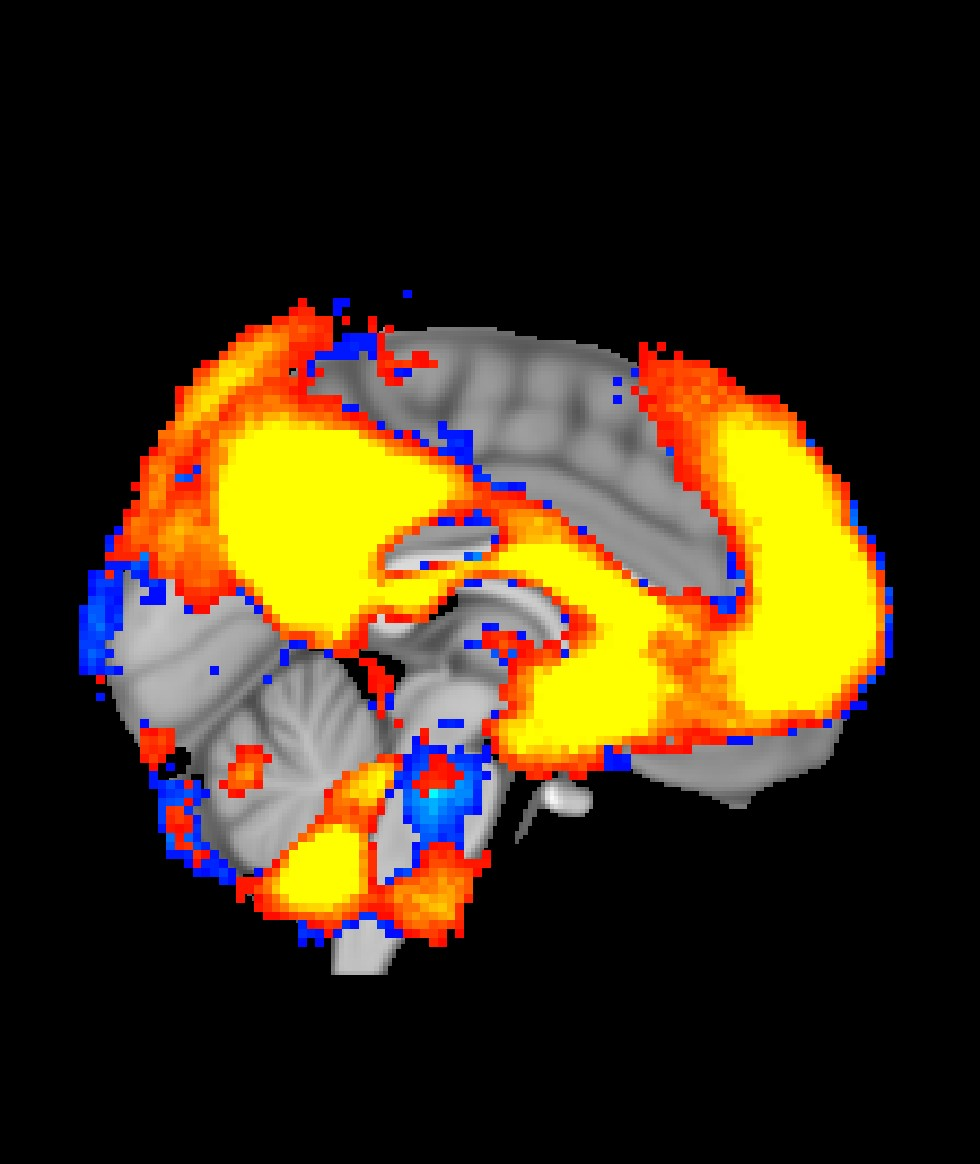
\includegraphics[width=.65\textwidth]{figures/Results/Neg_10-30}  
	\caption{An example component of signal, which is recognizable, isolated, and not corrupted by a substantial amount of noise. In this example, the signal is characterized as a strong and fairly isolated activation mainly in the parietal lobe and some in the temporal lobe.}
	\label{fig:res:diffpos} 
\end{figure}

\begin{figure}[H]                 
	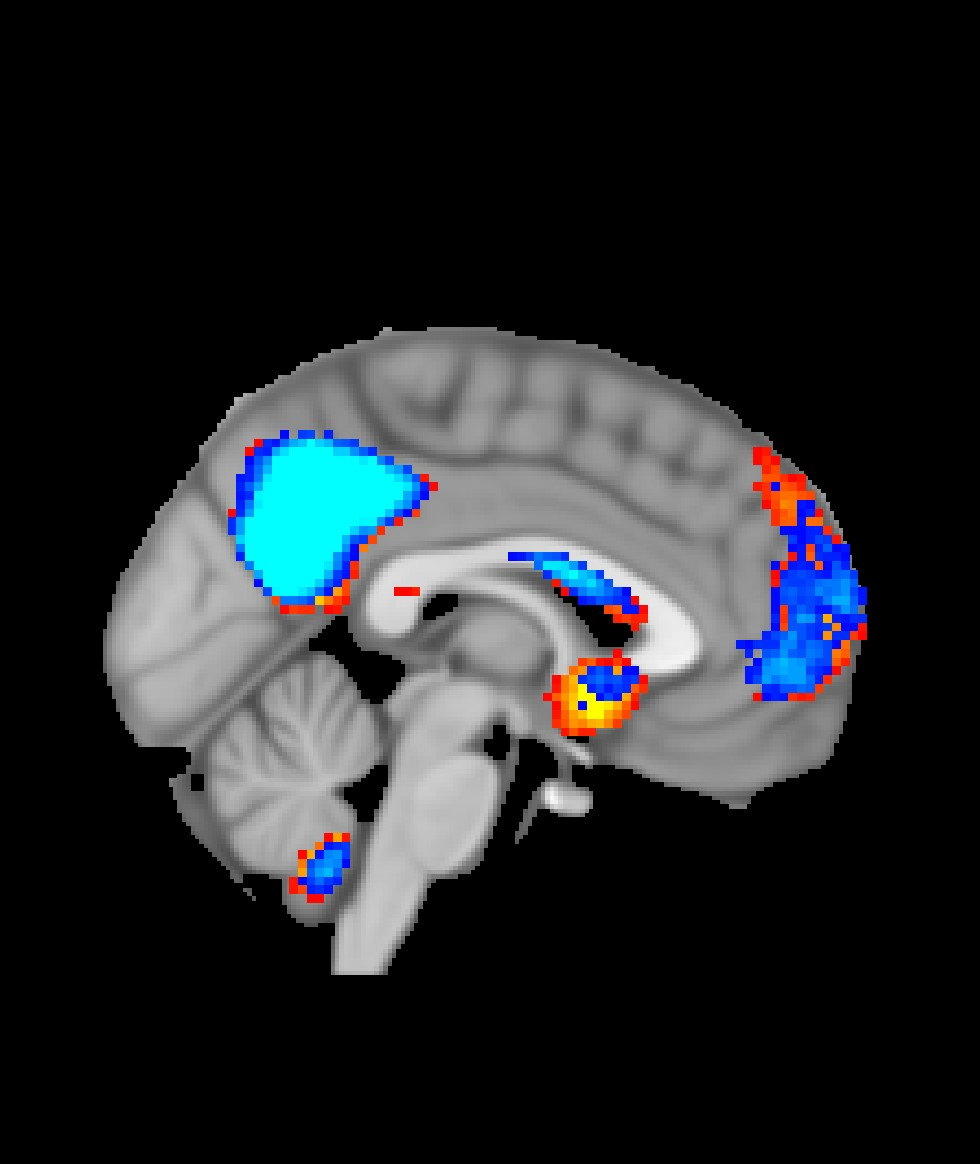
\includegraphics[width=.65\textwidth]{figures/Results/Neg_40-60}  
	\caption{An example component of signal, which is recognizable, isolated, and not corrupted by a substantial amount of noise. In this example, the signal is characterized as a strong and fairly isolated activation mainly in the parietal lobe and some in the temporal lobe.}
	\label{fig:res:diffneg} 
\end{figure}

\begin{figure}[H]                 
	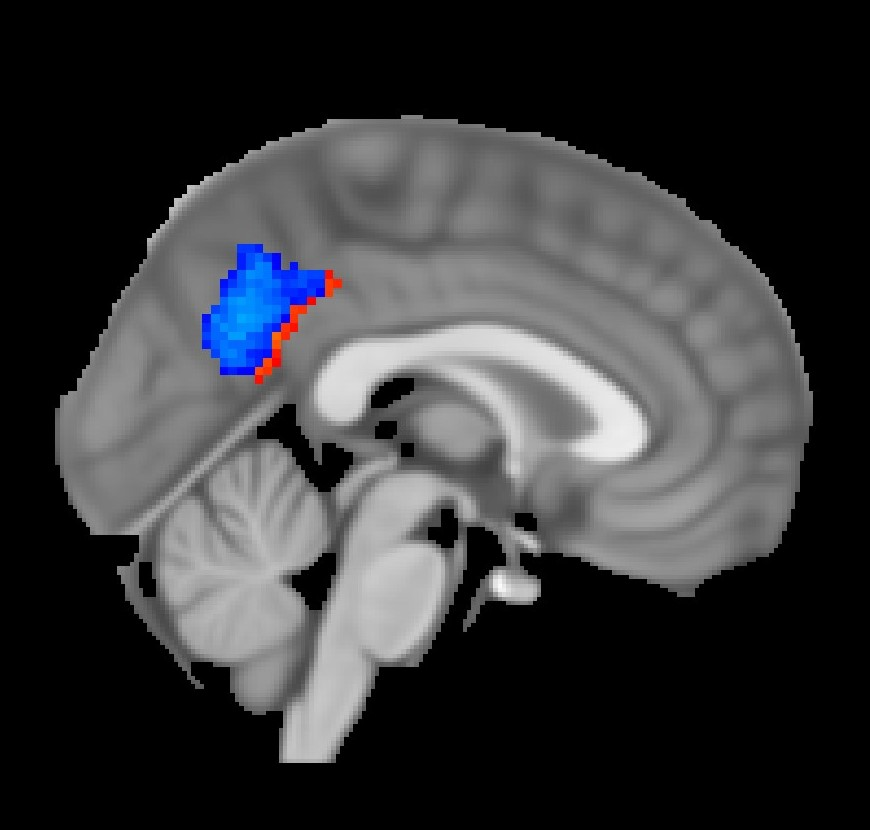
\includegraphics[width=.65\textwidth]{figures/Results/Neg_70-92}  
	\caption{An example component of signal, which is recognizable, isolated, and not corrupted by a substantial amount of noise. In this example, the signal is characterized as a strong and fairly isolated activation mainly in the parietal lobe and some in the temporal lobe.}
	\label{fig:res:diffneg} 
\end{figure}

\begin{figure}[H]                 
	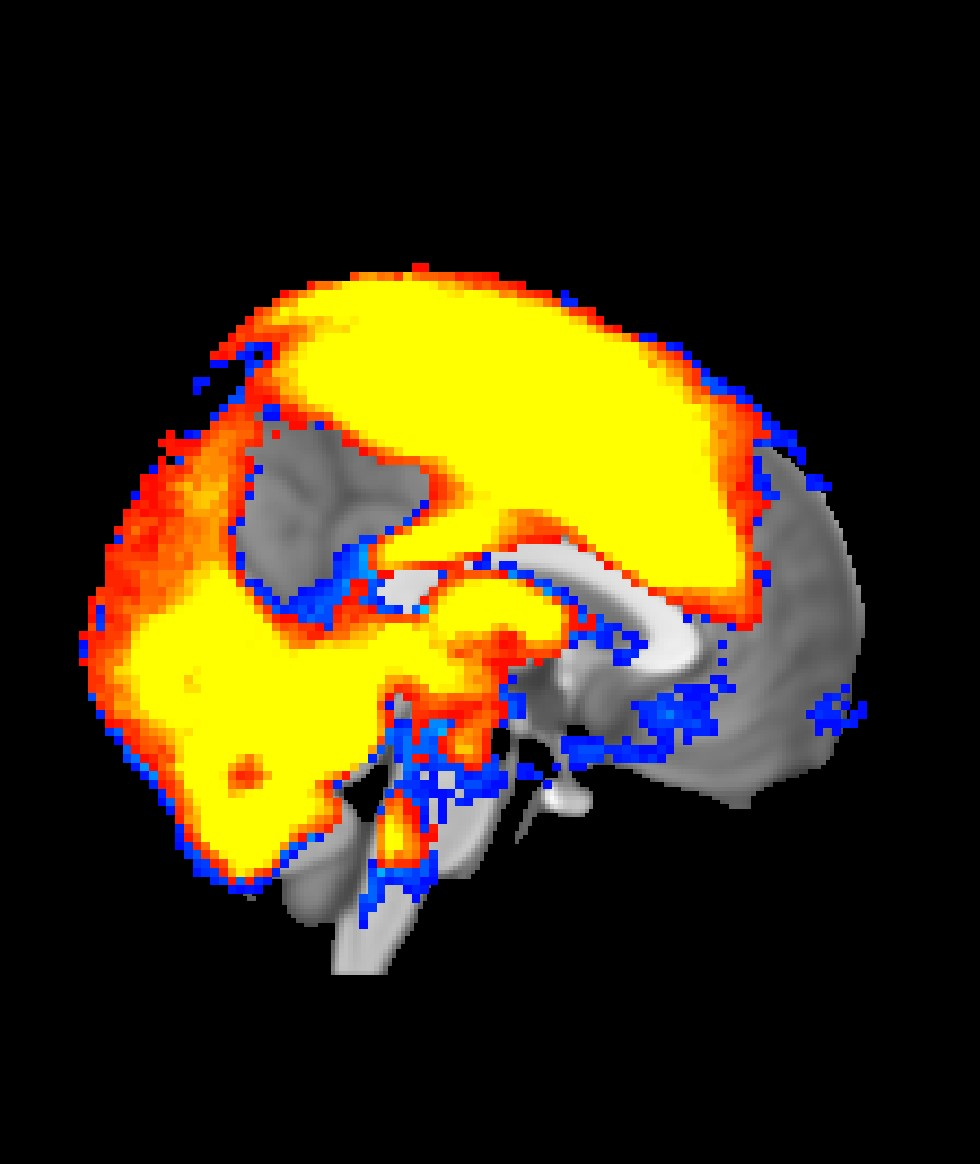
\includegraphics[width=.65\textwidth]{figures/Results/Pos_10-30}  
	\caption{An example component of signal, which is recognizable, isolated, and not corrupted by a substantial amount of noise. In this example, the signal is characterized as a strong and fairly isolated activation mainly in the parietal lobe and some in the temporal lobe.}
	\label{fig:res:diffpos} 
\end{figure}

\begin{figure}[H]                 
	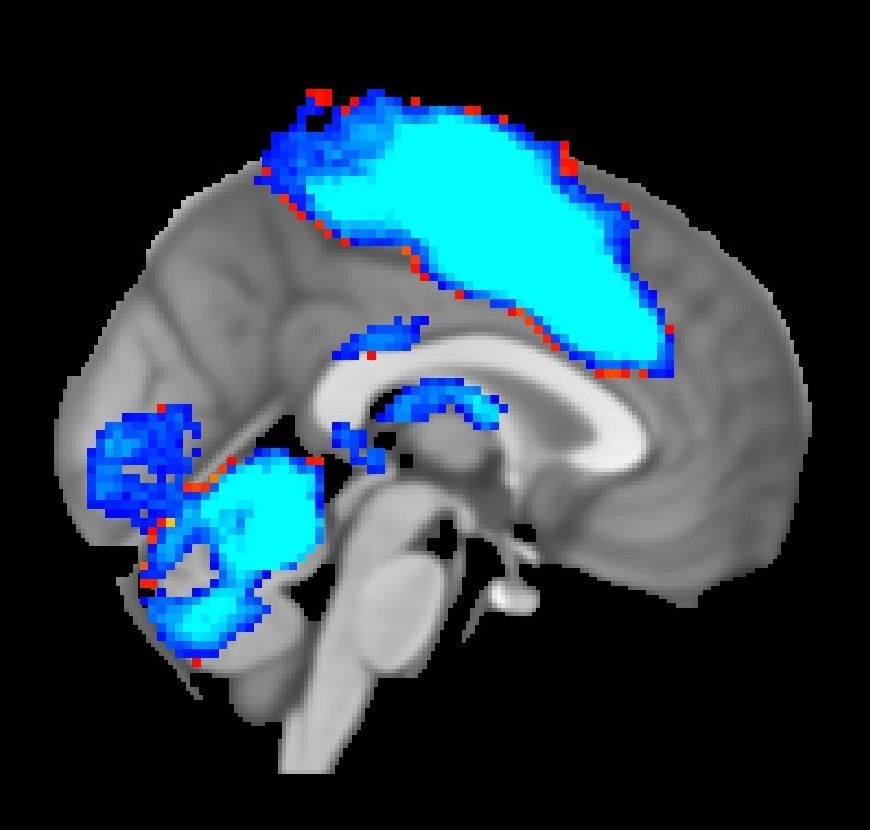
\includegraphics[width=.65\textwidth]{figures/Results/Pos_40-60}  
	\caption{An example component of signal, which is recognizable, isolated, and not corrupted by a substantial amount of noise. In this example, the signal is characterized as a strong and fairly isolated activation mainly in the parietal lobe and some in the temporal lobe.}
	\label{fig:res:diffneg} 
\end{figure}

\begin{figure}[H]                 
	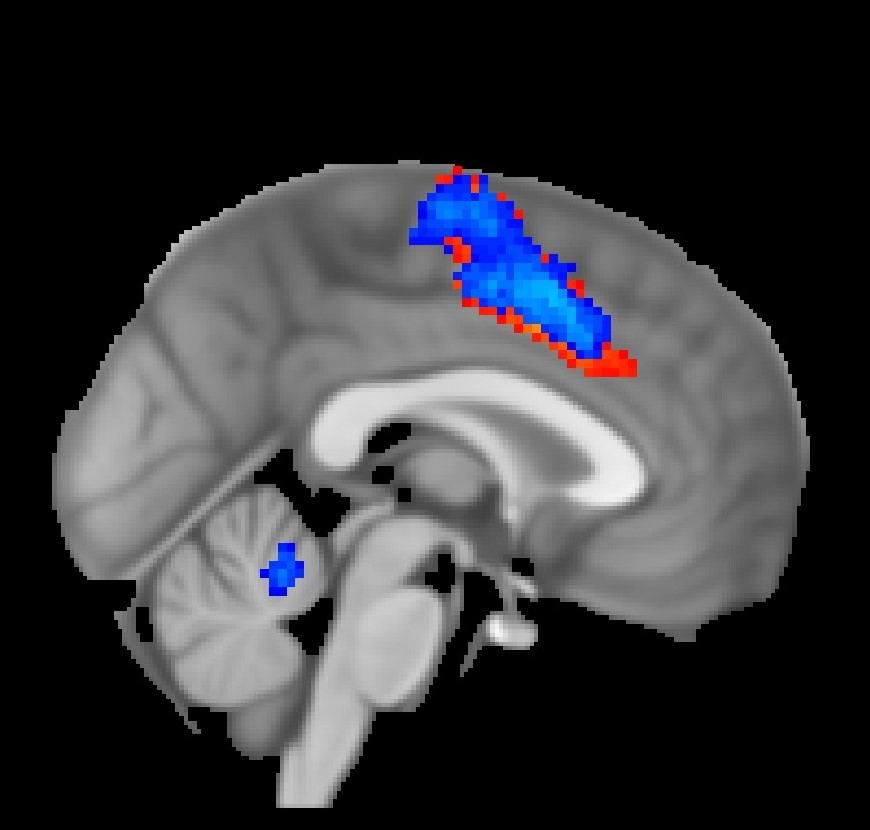
\includegraphics[width=.65\textwidth]{figures/Results/Pos_80-100}  
	\caption{An example component of signal, which is recognizable, isolated, and not corrupted by a substantial amount of noise. In this example, the signal is characterized as a strong and fairly isolated activation mainly in the parietal lobe and some in the temporal lobe.}
	\label{fig:res:diffneg} 
\end{figure}